%%%%%%%%%%%%%%%%%%%% author.tex %%%%%%%%%%%%%%%%%%%%%%%%%%%%%%%%%%%
%
% sample root file for your "contribution" to a contributed volume
%
% Use this file as a template for your own input.
%
%%%%%%%%%%%%%%%% Springer %%%%%%%%%%%%%%%%%%%%%%%%%%%%%%%%%%


% RECOMMENDED %%%%%%%%%%%%%%%%%%%%%%%%%%%%%%%%%%%%%%%%%%%%%%%%%%%
\documentclass[graybox]{svmult}

% choose options for [] as required from the list
% in the Reference Guide

\usepackage{type1cm}        % activate if the above 3 fonts are
                            % not available on your system
%
\usepackage{makeidx}         % allows index generation
\usepackage{graphicx}        % standard LaTeX graphics tool
                             % when including figure files
\usepackage{multicol}        % used for the two-column index
\usepackage[bottom]{footmisc}% places footnotes at page bottom


\usepackage{newtxtext}       % 
\usepackage[varvw]{newtxmath}       % selects Times Roman as basic font




\usepackage{comment}
\usepackage{graphicx}
\usepackage{tikz}
\usepackage{tikz-3dplot}
%\usepackage{caption}
\usepackage{subcaption}
%\usepackage{indentfirst}
\usepackage{float}
\usepackage{algpseudocode}
\usepackage{algorithm}
%\usepackage{braket}
\usepackage{commath}
\usepackage{url}
\usetikzlibrary{intersections, calc, math}


\algnewcommand\algorithmicforeach{\emph{for each}}
\algdef{S}[FOR]{ForEach}[1]{\algorithmicforeach\ #1\ \algorithmicdo}

\usetikzlibrary{angles,quotes}

\usetikzlibrary{shapes.geometric,arrows}
%
\tikzstyle{startstop} = [rectangle, rounded corners, text centered, draw=black, fill=blue!10]
\tikzstyle{process} = [rectangle, minimum width=2cm, minimum height=1cm, text centered, draw=black, fill=orange!10]
\tikzstyle{decision} = [diamond, aspect=3, minimum width=2cm, minimum height=1cm, text centered, draw=black, fill=red!10]
% define arrow style
\tikzstyle{compute} = [rectangle, minimum width=1cm, minimum height=1cm, text centered, draw=black, fill=green!10]
\tikzstyle{estimate} = [rectangle, rounded corners, minimum width=2cm, minimum height=1cm, text centered, draw=black, fill=yellow!10]
\tikzstyle{arrow} = [thick,->,>=stealth]

\usetikzlibrary{calc,arrows.meta,positioning,backgrounds}

%\usepackage[margin=15mm]{geometry}
%\usepackage{geometry}
\usepackage{bm}

\usepgfmodule{nonlineartransformations}
\makeatletter
\def\tikz@scan@transform@one@point#1{%
  \tikz@scan@one@point\pgf@process#1%
  \pgf@pos@transform{\pgf@x}{\pgf@y}}
\tikzset{%
  grid source opposite corners/.code args={#1and#2}{%
   \pgfextract@process\tikz@transform@source@southwest{%
     \tikz@scan@transform@one@point{#1}}%
   \pgfextract@process\tikz@transform@source@northeast{%
     \tikz@scan@transform@one@point{#2}}%
  },
  grid target corners/.code args={#1--#2--#3--#4}{%
   \pgfextract@process\tikz@transform@target@southwest{%
     \tikz@scan@transform@one@point{#1}}%
   \pgfextract@process\tikz@transform@target@southeast{%
     \tikz@scan@transform@one@point{#2}}%
   \pgfextract@process\tikz@transform@target@northeast{%
     \tikz@scan@transform@one@point{#3}}%
   \pgfextract@process\tikz@transform@target@northwest{%
     \tikz@scan@transform@one@point{#4}}%
  }
}

\def\tikzgridtransform{%
  \pgfextract@process\tikz@current@point{}%
  \pgf@process{%
    \pgfpointdiff{\tikz@transform@source@southwest}%
      {\tikz@transform@source@northeast}%
  }%
  \pgf@xc=\pgf@x\pgf@yc=\pgf@y%
  \pgf@process{%
    \pgfpointdiff{\tikz@transform@source@southwest}{\tikz@current@point}%
  }%
  \pgfmathparse{\pgf@x/\pgf@xc}\let\tikz@tx=\pgfmathresult%
  \pgfmathparse{\pgf@y/\pgf@yc}\let\tikz@ty=\pgfmathresult%
  %
  \pgfpointlineattime{\tikz@ty}{%
    \pgfpointlineattime{\tikz@tx}{\tikz@transform@target@southwest}%
      {\tikz@transform@target@southeast}}{%
    \pgfpointlineattime{\tikz@tx}{\tikz@transform@target@northwest}%
      {\tikz@transform@target@northeast}}%
}

\newcommand{\savedx}{0}
\newcommand{\savedy}{0}
\newcommand{\savedz}{0}

\newcommand{\somedrawing}%
{   \coordinate (a) at (-2,-2,-2);
    \coordinate (b) at (-2,-2,2);
    \coordinate (c) at (-2,2,-2);
    \coordinate (d) at (-2,2,2);
    \coordinate (e) at (2,-2,-2);
    \coordinate (f) at (2,-2,2);
    \coordinate (g) at (2,2,-2);
    \coordinate (h) at (2,2,2);
    \draw (a)--(b) (a)--(c) (a)--(e) (b)--(d) (b)--(f) (c)--(d) (c)--(g) (d)--(h) (e)--(f) (e)--(g) (f)--(h) (g)--(h);
    \fill (a) circle (0.1cm);
    \fill (d) ++(0.1cm,0.1cm) rectangle ++(-0.2cm,-0.2cm);
}

\newcommand{\rotateRPY}[4][0/0/0]% point to be saved to \savedxyz, roll, pitch, yaw
{   \pgfmathsetmacro{\rollangle}{#2}
    \pgfmathsetmacro{\pitchangle}{#3}
    \pgfmathsetmacro{\yawangle}{#4}

    % to what vector is the x unit vector transformed, and which 2D vector is this?
    \pgfmathsetmacro{\newxx}{cos(\yawangle)*cos(\pitchangle)}% a
    \pgfmathsetmacro{\newxy}{sin(\yawangle)*cos(\pitchangle)}% d
    \pgfmathsetmacro{\newxz}{-sin(\pitchangle)}% g
    \path (\newxx,\newxy,\newxz);
    \pgfgetlastxy{\nxx}{\nxy};

    % to what vector is the y unit vector transformed, and which 2D vector is this?
    \pgfmathsetmacro{\newyx}{cos(\yawangle)*sin(\pitchangle)*sin(\rollangle)-sin(\yawangle)*cos(\rollangle)}% b
    \pgfmathsetmacro{\newyy}{sin(\yawangle)*sin(\pitchangle)*sin(\rollangle)+ cos(\yawangle)*cos(\rollangle)}% e
    \pgfmathsetmacro{\newyz}{cos(\pitchangle)*sin(\rollangle)}% h
    \path (\newyx,\newyy,\newyz);
    \pgfgetlastxy{\nyx}{\nyy};

    % to what vector is the z unit vector transformed, and which 2D vector is this?
    \pgfmathsetmacro{\newzx}{cos(\yawangle)*sin(\pitchangle)*cos(\rollangle)+ sin(\yawangle)*sin(\rollangle)}
    \pgfmathsetmacro{\newzy}{sin(\yawangle)*sin(\pitchangle)*cos(\rollangle)-cos(\yawangle)*sin(\rollangle)}
    \pgfmathsetmacro{\newzz}{cos(\pitchangle)*cos(\rollangle)}
    \path (\newzx,\newzy,\newzz);
    \pgfgetlastxy{\nzx}{\nzy};

    % transform the point given by #1
    \foreach \x/\y/\z in {#1}
    {   \pgfmathsetmacro{\transformedx}{\x*\newxx+\y*\newyx+\z*\newzx}
        \pgfmathsetmacro{\transformedy}{\x*\newxy+\y*\newyy+\z*\newzy}
        \pgfmathsetmacro{\transformedz}{\x*\newxz+\y*\newyz+\z*\newzz}
        \xdef\savedx{\transformedx}
        \xdef\savedy{\transformedy}
        \xdef\savedz{\transformedz}     
    }
}

\tikzset{RPY/.style={x={(\nxx,\nxy)},y={(\nyx,\nyy)},z={(\nzx,\nzy)}}}

\newcommand{\MarkRightAngle}[4][1.0cm]% #1=size (optional), #2-#4 three points: \angle #2#3#4
{\coordinate (tempa) at ($(#3)!#1!(#2)$);
 \coordinate (tempb) at ($(#3)!#1!(#4)$);
 \coordinate (tempc) at ($(tempa)!0.5!(tempb)$);%midpoint
 \draw (tempa) -- ($(#3)!2!(tempc)$) -- (tempb);
} 
%%%%%%%%%%%%%%%%%%%%%%%%%%%%%%%%%%%%%%%%%%%%%%%%%%%%%%%%%%%%%%%%%%%%


\graphicspath{ {./img/}}

\begin{document}

\title*{Moving Object 3D Detection and Segmentation \\
Using Optical Flow Clustering}
% Use \titlerunning{Short Title} for an abbreviated version of
% your contribution title if the original one is too long
\author{Dmitriy Zhuravlev}
% Use \authorrunning{Short Title} for an abbreviated version of
% your contribution title if the original one is too long
\authorrunning{Moving Object 3D Detection}
\institute{D. Zhuravlev \at Taras Shevchenko National University of Kyiv, \email{dzhuravlev@ukr.net}}
%\and Name of Second Author \at Name, Address of Institute \email{name@email.address}}
%
% Use the package "url.sty" to avoid
% problems with special characters
% used in your e-mail or web address
%
\maketitle

\abstract*{Deep learning methods have recently improved the performance and accuracy of prediction using big data and abundant computing resources.
However, many complex problems in Computer Vision, including 3D detection, motion estimation, and image segmentation, cannot be easily solved.
But it is still possible to benefit from using "traditional" methods.\\
This article analyzes the relationship between Optical Flow  and object localization.
%This paper describes a detection and localization method based on Optical Flow Clustering.
The proposed algorithm works with moving objects and performs not only instance segmentation but also determines the type of objects and estimates 3D bounding boxes using geometric constraints.
Since the method is based only on classical Computer Vision techniques it does not require data and time for the training process and can be deployed on constrained devices.}

\abstract{ 
Deep learning methods have recently improved the performance and accuracy of prediction using big data and abundant computing resources.
However, many complex problems in Computer Vision, including 3D detection, motion estimation, and image segmentation, cannot be easily solved.
All the same, it is still possible to benefit from using `traditional' methods.\\
This article analyzes the relationship between optical flow  and object localization.
%This paper describes a detection and localization method based on Optical Flow Clustering.
The proposed algorithm works with moving objects and performs not only instance segmentation but also determines the type of objects and estimates 3D bounding boxes using geometric constraints.
Since the method is based only on an algorithmic understanding of three-dimensional data, it does not require data and time for the training process and can be deployed on constrained devices.}

%
\section{Introduction}
\label{sec:1}
Moving object detection and segmentation is an important task in many  \emph{Computer Vision} (CV)  applications such as surveillance, autonomous driving, and robotics. The ability to accurately detect and segment moving objects is crucial for tasks such as tracking, path planning, obstacle avoidance, and behavior analysis. Traditional 2D object detection methods have limitations when dealing with occlusions, dynamic backgrounds, and changes in lighting and appearance. 3D object localization can provide more accurate and robust results, but it is a challenging task that often requires the integration of multiple sensing modalities. Developing accurate and efficient  methods for moving object 3D detection and segmentation can have a significant impact on various domains including transportation, security, and entertainment.


% and has important applications in locating personnel and/or equipment in large open spaces such as a farm or a mine.
%Detection of 3D objects in real-time is a widely demanded task of \emph{Computer Vision} (CV).
Especially important is the ability to determine the location without the use of additional equipment  \cite{lidar,3d_cam}
but only with the help of a monocular camera due to its cheapness.
While there are limitations to using such cameras, including limited depth perception, researchers are actively developing new algorithms and techniques to address these challenges and improve the accuracy and robustness of 3D object detection using monocular cameras.

%However, owing to the fact that such a camera does not provide information 
%about the distance to the object, this task is difficult.

Nowadays, deep learning methods have shown great promise in recent years for 3D object detection, particularly with the advent of new 3D sensing technologies and datasets.
These methods~\cite{yolo_paper,traffic} typically rely on convolutional neural networks (CNNs) and other deep learning architectures to automatically learn features and representations from the data. However, deep learning methods may require a large amount of labeled data to train, and can be computationally intensive and difficult to optimize.
Also, in the end, it is hard to guarantee that the trained model will perform equally well with any data.

On the contrary, methods \cite{3d_geom,lift} based on classical CV use mathematical operations on extracted features  and geometrical constraints to minimize prediction errors. These methods can be effective in certain scenarios, such as when the objects have well-defined geometric shapes and the scene is well-structured. This gives confidence that the system will behave the same with any data, and does not require training time and data. Also, it remains available for deployment on low-cost microcontrollers.

%The article proposes a solution to the problem using only classical Computer Vision (CV) methods.
%That allows not only to use them on constrained devices but also avoids excessive costs of training and using Neural Networks.

We will describe the relationship between object localization and  movement to provide a joint method for 3D detection and instance segmentation.
The main contribution of this paper can be summarized as follows:
\begin{itemize}

    \item  a method for the estimation of the object orientation by using Optical Flow clustering;
    \item  an approach for the determination of an object type from the corresponding instance segmentation;
    \item  a technique for the construction of a 3D box  based on the object  orientation and  type;
    \item an algorithm for instance segmentation based on 3D localization;
    \item a design of the end-to-end baseline architecture that provides good performance with high accuracy;
    \item open-sourced PoC implementation, available for
download at \url{https://github.com/DmitriyZhuravlev/3dim-optical-flow}%{\textbf{https://github.com/DmitriyZhuravlev/3dim-optical-flow}}

\end{itemize}

The rest of this paper is organized as follows. In the next section,
a review of popular methods of segmentation and object detection is given. 
Sect.~\ref{sec:back}  introduces a set of necessary concepts that will be used later in our method from Sect.~\ref{sec:meth}.
The results of real-world testing with a concluding summary are presented in Sect.~\ref{sec:conc}.








\section{Related Studies}
In this section, we discuss the most relevant work on object detection and instance segmentation.
Due to the fact that the proposed  method uses both of them inseparably, we first address previous work in the area of motion segmentation.  Subsequently, we attempt to summarize the most relevant work on existing methods for 3D localization that intend to recreate the depth information from an RGB image.\\
However, in our work, these methods complement each other, so the goals and methods of the previous studies are principally different from the scope of this paper. This paper is assumed the natural continuation of the previous~\cite{lift} with removing 2D detector dependency. 
\subsection{Video Segmentation}
Semantic object segmentation is a crucial first step in video understanding  applications for video search and retrieval purposes. 
Therefore, finding reliable solutions has become an active research problem.
While segmentation methods have made significant progress in recent years, there are still several limitations and challenges that need to be addressed to improve the accuracy, efficiency, and generalizability of segmentation models.

Methods for segmenting video objects are aimed at
automatic object extraction from video. These
methods use features such as clustering of point trajectories~\cite{segm_trajec,segm_tracing}, motion characteristics~\cite{segm_visual}, appearance~\cite{segm_key,segm_graph} to achieve object segmentation.
Recently, in~\cite{segm_prim}, the main object was separated from the background in the video based on the scheme of variable convex optimization.
Also, in the article~\cite{segm_fusion}  end-to-end learning structure
combining motion and appearance information is proposed in order to create
binary segmentation by pixels for each frame.

Standard approaches to the problem include trajectory analysis and appearance-based methods. Several studies~\cite{segm_chain,segm_clust} have shown a significant improvement in the use of a stream of visual features for object segmentation.
Previous research has shown that a simple clustering technique can be used for semantic segmentation. However, this
requires human intervention to estimate the amount of
clusters by watching a short video clip.

Since semantic segmentation and motion segmentation do not
separate instances of objects, a segment can consist of several objects.
In order to extract individual objects, methods use a pre-trained object detection model \cite{fusionseg} as its backbone.

The above methods either cannot separate one object from another or use object detection for this, whereas the proposed method uses its own 3D estimation. 

\subsection{Monocular 3D Object Detection}
This part of the article discusses the existing methods of 3D localization that intend to recreate the depth information from a monocular image.

Like most of the works related to 3D object detection from a single image, \cite{3d_geom} proposed a method for regression of an observation angle and 3D object sizes from the cropped image patch enclosed by 2D detection box. Using the regressed dimensions and orientations of the 3D box and 2D detection box, they try to minimize the re-projection error related to the initial 2D detection box constraints.
Since each side of the 2D detection box can correspond to any of the eight corners of the 3D box, there are $8^4$ configurations.


In the \cite{3d_geom_reduced} the number of plausible configurations is reduced to $64$.
These configurations go through equations to find the vertices of a cuboid and the resulting solutions are ranked by approximation error or intersection over union (IoU) score between the tightest bounding box for the projected vertices of the fitted cuboid and the 2D detection rectangle.

%there are many options from which you need to choose the best, which does not allow using these methods in real-time applications.

To simplify object distance measurement, the Bird's Eye View (BEV) based architecture is proposed in  
\cite{bev_1} for vehicle detection with uncalibrated traffic cameras. Since all traffic participants are in contact with the ground, the distance can be estimated as the detection of points of contact of the vehicle with the road. The proposed method involves two stages: motion cancellation and the detection of position, size,
and orientation using convolutional neural networks. In this work, two types of detectors for rotated box prediction on BEV are proposed.
The one-stage detectors have the advantage of fast operating speed because of the direct prediction of the bounding box from the feature map grid without refinement.
On the other hand, two-stage detectors predict the position and size of the object more precisely since the network predicts the box proposal and performs refinement in two steps.
However, such defectors operate slower.


\cite{bev_2} extends the previous approach for uncalibrated traffic cameras using dual-view architecture.
In this architecture, both the original view and BEV images are taken as input. The original view feature maps are warped
to BEV and concatenated with BEV feature maps. The dual-view structure enables feature learning before warping, where the object shapes are regular and the
knowledge propagation is easier, but it still has the two-stage detectors issues.


In \cite{bev_mod} the idea of learning moving object detection directly in BEV space is explored. 
The architecture based on two-stream RGB and optical flow fusion is proposed for object localization.
However, the lengths of some objects are not captured perfectly and some of the objects are misclassified as false static objects, which shows that there is still room for
improvement.

All the mentioned methods study 3D object localization using different neural networks which not only get a 2D box but also extract additional information from the image to predict the distance and orientation.
However, the geometric constraints of moving objects are not explored thoroughly enough. 
In this work, we identify real-world scenarios where high reconstruction accuracy is guaranteed via geometric analysis and apply our algorithm to localize 3D objects in real-time.


\section{Background} \label{sec:back}
\subsection{Camera Model}
\begin{comment}

\begin{figure}%[H]
\centering
\tdplotsetmaincoords{-60}{-35}
\begin{tikzpicture}
  [
    tdplot_main_coords,
    >=Stealth,
    my dashed/.style={dashed, thick, ->, shorten >=-15pt, shorten <=-15pt, every node/.append style={font=\footnotesize}},
    my box/.style={thin, gray!70},
    my blue/.style={blue, line cap=round, -{Triangle[width=3*#1]}, line width=#1, shorten >=#1*1.75pt, every node/.append style={fill, circle, inner sep=0pt, minimum size=#1*3.5pt, anchor=center, outer sep=0pt}},
    my label/.append style={midway, font=\scriptsize},
    my vectors/.style={green!50!black, {Stealth[scale=.75]}-{Stealth[scale=.75]}},
    my red/.style={thick, red, line cap=round},
    my grey/.style={gray!70},
    description/.style={draw=gray!70, thick, line cap=round, every node/.style={align=center, font=\scriptsize\sffamily, anchor=north}},
  ]
%   \draw [help lines] (-2,0,0) -- (2,0,0) node[anchor=north west]{$x$} (0,0,0) -- (0,7,0) node[anchor=north east]{$y$} (0,0,0) -- (0,0,2) node[anchor=north]{$z$} (-2,7,0) -- (2,7,0);
  \draw [my grey] (0,4,0) -- (0,7,0) (-2,7,0) -- (2,7,0);
  \coordinate (o) at (0,0,0);
  \path [draw=gray!70, text=gray, fill=gray!20, opacity=0.8, text opacity=1] (-1.5,4,1.75) coordinate (a) -- ++(0,0,-3.5) coordinate (b) -- ++(3,0,0) coordinate (c) -- ++(0,0,3.5) coordinate (d) -- cycle node [pos=.95, above, sloped, anchor=south west] {$z=f$} ;
%   \foreach \i in {a,b,c,d} \node [red, font=\scriptsize] at (\i) {\i};
  \draw [my grey] (-2,0,0) -- (2,0,0) (0,0,0) -- (0,4,0) (0,0,0) -- (0,0,2);
  \draw [thick, ->, every node/.style={font=\footnotesize, inner sep=0pt}] (o) node [anchor=north west] {$O_c$} (o) edge node [pos=1, anchor=north east] {$z_c$} ++(0,1,0) edge node [pos=1, anchor=north] {$y_c$} ++(0,0,1) -- ++(1,0,0) node [anchor=north west] {$x_c$};
  \draw [my box] (o) ++(0,4,-.5) coordinate (p1) -- ++(1,0,0) coordinate (p2) -- ++(0,0,-1.25) coordinate (p3);
  \foreach \i in {0,1,...,4} \draw [my box] (p1) ++(\i*.25,0,0) -- ++(0,0,-.25);
  \foreach \i in {0,1,...,5} \draw [my box] (p2) ++(0,0,-\i*.25) -- ++(-.25,0,0);
  \draw [my box] (p1) ++(0,0,-.25) -- ++(.75,0,0) -- ++(0,0,-1);
  \draw [my dashed, cyan] ($(b)!1/2!(c)$) -- ($(d)!1/2!(a)$) node [below=15pt, anchor=north] {$y$};
  \draw [my dashed, cyan] ($(b)!1/2!(a)$) -- ($(d)!1/2!(c)$) node [above right=17pt, anchor=north west] {$x$};
  \draw [my dashed, green!50!black, <->] (a) node [below=15pt, anchor=north] {$v$} -- (b) -- (c) node [above right=17pt, anchor=north west] {$u$};
  \path [green!50!black, every node/.style={font=\scriptsize, inner sep=0pt}] (p2) node [above right, anchor=south west] {$(u,v)$};
  \path (p2) ++(-.125,0,0) coordinate (q2) ++(0,0,-.125) coordinate (r2);
  \draw [my blue=1] ($(0,4,0)+($(q2)-(p1)$)$) coordinate (s2) -- (r2) node (d1) {};
  \scoped[on background layer]{\draw [my blue=1.75] ($($1.75*($(s2)-(0,4,0)$)$)+(0,7,0)$) -- ++($1.75*($(r2)-(s2)$)$) node (d2) [label={[label distance=-20pt]above:{$p=(x,y,z)$}}] {};}
  \draw [my vectors] (0,4,.1) -- ($(s2)+(0,0,.1)$) node [below, my label, sloped] {$\vec{u}$};
  \draw [my vectors] (-.1,4,0) -- ($(q2)-(s2)+(-.1,4,0)$) node [left, my label] {$\vec{v}$};
  \draw [my red] (o) -- (d1.center);
  \scoped[on background layer]{\draw [my red] (d1.center) -- (d2.center);}
  \path [description] (0,4,0) [out=-95, in=95] to (-.75,4,.25) node {principal\\point} (0,6.5,0) [out=-95, in=95] to (-.75,6.5,.25) node {optical\\axis};
\end{tikzpicture}
\caption{Pinhole camera model.}
\label{fig:camera}
\end{figure}
\end{comment}

The camera model is a basis for developing a computer vision application. We use the Pinhole model with no distortion factor to describe the projection of 3D points onto an image plane. % as shown in the Figure~\ref{fig:camera}.\\

\begin{figure}%[H]
\centering
\tdplotsetmaincoords{-60}{-35}
\begin{tikzpicture}
  [
    tdplot_main_coords,
    >=Stealth,
    my dashed/.style={dashed, thick, ->, shorten >=-15pt, shorten <=-15pt, every node/.append style={font=\footnotesize}},
    my box/.style={thin, gray!70},
    my blue/.style={blue, line cap=round, -{Triangle[width=3*#1]}, line width=#1, shorten >=#1*1.75pt, every node/.append style={fill, circle, inner sep=0pt, minimum size=#1*3.5pt, anchor=center, outer sep=0pt}},
    my label/.append style={midway, font=\scriptsize},
    my vectors/.style={green!50!black, {Stealth[scale=.75]}-{Stealth[scale=.75]}},
    my red/.style={thick, red, line cap=round},
    my grey/.style={gray!70},
    description/.style={draw=gray!70, thick, line cap=round, every node/.style={align=center, font=\scriptsize\sffamily, anchor=north}},
  ]
%   \draw [help lines] (-2,0,0) -- (2,0,0) node[anchor=north west]{$x$} (0,0,0) -- (0,7,0) node[anchor=north east]{$y$} (0,0,0) -- (0,0,2) node[anchor=north]{$z$} (-2,7,0) -- (2,7,0);
  \draw [my grey] (0,4,0) -- (0,7,0) (-2,7,0) -- (2,7,0);
  \coordinate (o) at (0,0,0);
  \path [draw=gray!70, text=gray, fill=gray!20, opacity=0.8, text opacity=1] (-1.5,4,1.75) coordinate (a) -- ++(0,0,-3.5) coordinate (b) -- ++(3,0,0) coordinate (c) -- ++(0,0,3.5) coordinate (d) -- cycle node [pos=.95, above, sloped, anchor=south west] {$z=f$} ;
%   \foreach \i in {a,b,c,d} \node [red, font=\scriptsize] at (\i) {\i};
  \draw [my grey] (-2,0,0) -- (2,0,0) (0,0,0) -- (0,4,0) (0,0,0) -- (0,0,2);
  \draw [thick, ->, every node/.style={font=\footnotesize, inner sep=0pt}] (o) node [anchor=north west] {$O_c$} (o) edge node [pos=1, anchor=north east] {$z_c$} ++(0,1,0) edge node [pos=1, anchor=north] {$y_c$} ++(0,0,1) -- ++(1,0,0) node [anchor=north west] {$x_c$};
  \draw [my box] (o) ++(0,4,-.5) coordinate (p1) -- ++(1,0,0) coordinate (p2) -- ++(0,0,-1.25) coordinate (p3);
  \foreach \i in {0,1,...,4} \draw [my box] (p1) ++(\i*.25,0,0) -- ++(0,0,-.25);
  \foreach \i in {0,1,...,5} \draw [my box] (p2) ++(0,0,-\i*.25) -- ++(-.25,0,0);
  \draw [my box] (p1) ++(0,0,-.25) -- ++(.75,0,0) -- ++(0,0,-1);
  \draw [my dashed, cyan] ($(b)!1/2!(c)$) -- ($(d)!1/2!(a)$) node [below=15pt, anchor=north] {$y$};
  \draw [my dashed, cyan] ($(b)!1/2!(a)$) -- ($(d)!1/2!(c)$) node [above right=17pt, anchor=north west] {$x$};
  \draw [my dashed, green!50!black, <->] (a) node [below=15pt, anchor=north] {$v$} -- (b) -- (c) node [above right=17pt, anchor=north west] {$u$};
  \path [green!50!black, every node/.style={font=\scriptsize, inner sep=0pt}] (p2) node [above right, anchor=south west] {$(u,v)$};
  \path (p2) ++(-.125,0,0) coordinate (q2) ++(0,0,-.125) coordinate (r2);
  \draw [my blue=1] ($(0,4,0)+($(q2)-(p1)$)$) coordinate (s2) -- (r2) node (d1) {};
  \scoped[on background layer]{\draw [my blue=1.75] ($($1.75*($(s2)-(0,4,0)$)$)+(0,7,0)$) -- ++($1.75*($(r2)-(s2)$)$) node (d2) [label={[label distance=-20pt]above:{$p=(x,y,z)$}}] {};}
  \draw [my vectors] (0,4,.1) -- ($(s2)+(0,0,.1)$) node [below, my label, sloped] {$\vec{u}$};
  \draw [my vectors] (-.1,4,0) -- ($(q2)-(s2)+(-.1,4,0)$) node [left, my label] {$\vec{v}$};
  \draw [my red] (o) -- (d1.center);
  \scoped[on background layer]{\draw [my red] (d1.center) -- (d2.center);}
  \path [description] (0,4,0) [out=-95, in=95] to (-.75,4,.25) node {principal\\point} (0,6.5,0) [out=-95, in=95] to (-.75,6.5,.25) node {optical\\axis};
\end{tikzpicture}
\caption{Pinhole camera model}
\label{fig:camera}
\end{figure}

In this model, the image plane is positioned a fixed distance behind the camera's optical center as shown in Fig.~\ref{fig:camera}. The relationship between a point in 3D space and its projection onto the image plane is defined by a set of equations, which take into account the focal length of the camera lens, the position of the point relative to the camera's optical center, and the orientation of the camera relative to the scene.


Let us describe the correspondences between the camera, world, and picture coordinate systems.
Let $p = (x_1^w, x_2^w, x_3^w)$ be a 3D point in the world coordinate system.
It can be transformed into camera coordinates using the \emph{extrinsic matrix} which consists of the rotation $\emph{R} \in \mathbb{SO}(3)$  and translation $\emph{t} \in \mathbb{R}^3$ between the two coordinate systems:
    $$
     \begin{bmatrix}
	 x_1^c\\x_2^c\\x_3^c		
	 \end{bmatrix}
	 =
	 \emph{R}
	 \begin{bmatrix}
	 x_1^w\\x_2^w\\x_3^w		
	 \end{bmatrix}
	 + \emph{t}
	 \label{eq:wc} \; .
$$

The new 3D point in the camera coordinate system is projected onto the image plane using the \emph{intrinsic matrix} $\emph{K}$ which consists of internal camera parameters like the focal length, optical center, etc. : 
$$
\begin{bmatrix}
		u'\\v'\\w'
		\end{bmatrix}=		
		 \emph{K}
		\begin{bmatrix}
		x_1^{c}\\x_2^{c}\\x_3^{c}
		\end{bmatrix}
    \label{eq:k1} \; ,
$$
where $u = \frac{u'}{w'}$ \;,  \; $v = \frac{v'}{w'}$ \;.\\
The overall projection in homogeneous coordinates can be expressed by:
$$ \begin{bmatrix}
		u'\\v'\\w'
		\end{bmatrix}=
		\emph{K} \left(\emph{R}
		\begin{bmatrix}
	    x_1^w\\x_2^w\\x_3^w		
	    \end{bmatrix}
		+ \emph{t} \right) \; .$$ % as shown in  Figure~\ref{fig:camera}.

\subsection{Optical Flow}
\emph{Optical Flow} (OF) is a technique used to estimate the motion of objects in a video sequence. It is based on the assumption that pixels in an image sequence move smoothly over time and that their motion can be represented as a 2D vector field.


The OF algorithm works by analyzing the brightness pattern of pixels in successive frames of a video sequence. The algorithm assumes that the intensity of a pixel should remain constant over time, so any changes in intensity must be due to motion: 
$I(p, t) = I(p + u, t + 1) $
where $I(p, t)$ is image intensity as a function of space $x = (x_1, x_2)$ and time $t$, and $u = (u_1, u_2)$ is the 2D velocity.

Several different approaches to motion estimation have been proposed. For example,
the Horn-Schunk method~\cite{horn}. It assumes that the optical flow is smooth over the entire image and computes an estimate of the velocity field by an equation minimization:
\[
E = \int \!\!\! \int \bigl(I_{x_1}u_1 + I_{x_2}u_2 + I_t\bigr)^2 dx_1dx_2 + \alpha \int \!\!\! \int \biggl(\frac{\partial u_1}{\partial x_1}^2 + \frac{\partial u_1}{\partial x_2}^2 + \frac{\partial u_2}{\partial x_1}^2 + \frac{\partial u_2}{\partial x_2}^2\biggr)dx_1dx_2
\]
where $\alpha$ is the smoothness term of the velocity field and
$\frac{\partial u_1}{\partial x_1}$ and 
$\frac{\partial u_2}{\partial x_1}$
are the partial derivatives of the optical velocity component~$u$. The $\alpha$ regularization parameter controls the rate of the smoothness constraint. 
\begin{comment}

The Horn-Schunck method minimizes the previous equation to obtain the velocity field, $[u\ v]$, for each pixel in the image, which is given by the following equations:
\begin{align*}
u^{k+1}_{x,y} &= \bar{u}^{k}_{x,y} - 
\frac{I_x[I_x \bar{u}^{k}_{x,y} + I_y\bar{v}^{k}_{x,y} 
+ I_t]}{\alpha^2 + I_x^2 + I_y^2}\\
v^{k+1}_{x,y} &= \bar{v}^{k}_{x,y} - 
\frac{I_y[I_x\bar{u}^{k}_{x,y} + I_y\bar{v}^{k}_{x,y} 
+ I_t]}{\alpha^2 + I_x^2 + I_y^2}
\end{align*}

\end{comment}
\subsection{Segmentation}
Image segmentation is the process of dividing an image into
its constituent areas or objects. Subdivision-level
images depend on the problem being solved. The segmentation process can stop when the objects of interest are isolated for further processing.

The result of image segmentation is a set of segments that collectively cover the entire image or a set of edges extracted from an image. Each of the pixels in an area has some characteristic or computed property such as color, intensity, or texture.

Let the function $g(x,y) \in \mathbb{R}^3$ represent an RGB color at any point $(x,y)$  of domain $\Omega \in  \mathbb{R}^2$ where an image is captured.
%Image is then defined as  $g = \{(x,y)|(x,y) \in \mathbb{R}^2\}$. The RGB color representation of an image is mathematically represented by $g(x,y) \in \mathbb{R}^3$. 
The aim is to find regions 
${\Omega}_1, {\Omega}_2, \ldots, {\Omega}_n $ for  $n \in N$, of a domain $\Omega \in \mathbb{R}^2$, corresponding to different $n$ objects or their parts or shadows in the image. 

\begin{comment}
    

The segmentation problem has the following definition: Suppose $\Omega$ is a domain of 
$h$, find ${\Omega}_1, {\Omega}_2, \ldots, {\Omega}_n $
 such that
 \[ \Omega = \cup_{i=1}^n \Omega_i, \]
 and $g$  varies smoothly over the regions $\Omega_i$, $i=1,2, \ldots, n$, but discontinuously over the boundaries between the regions.


In terms of approximation theory, we can represent it as finding an approximation 
$f$ of $g$  in such a way that each $f_i$ represents the region $\Omega_i$  via a piece-wise smooth function.
\end{comment}


Segmentation can be achieved by several methods, which include thresholding-based, edge-based, region-based, and clustering techniques.

\subsection{Clustering}

Clustering is a data analysis technique for separating a data set into subgroups of related data. K-means~\cite{kmeans} is one of the most widely used unsupervised clustering methods.

In the clustering problem, it is required to group  a set $\{x_1, \ldots, x_m \}$ into several connected \emph{clusters}. Here are the feature vectors for each data point $x_i \in \mathbb{R}^n$ but without the labels  (making this an unsupervised learning problem).
The goal of the algorithm is to predict $k$ centroids and label $c_i$ for each data point.

The classical algorithm can be expressed as an optimization problem:
$$
\mathcal{U}^* =
\underset{U\in\mathcal{P}}{\mathrm{argmin}} ~\,\max_{c_k\in\chi} 
\sum_{k=1}^C \sum_{i=1}^n
U_{k,i} ||c_k - x_i||_d^2
$$
for some distance $||\cdot||_d$, membership matrix $U$ (which assigns clusters to each $x$, $c_k$ is the $k$-th cluster center, and $x_j$ is the $j$-th data point. Principally, $U_{i,k}$ is $1$ if $x_i$ is in the $k$-th cluster and $0$ otherwise. The summations compute the total distance of each data point to its cluster center.

Let us denote this algorithm by $\mathrm{KMEANS}$ for further use in the proposed algorithm.
%for segmentation of the optical flow vectors. %Some examples can be found in Fig.~\ref{fig:clust}.

\subsection{Inverse Perspective Mapping}
\emph{Inverse Perspective Mapping} (IPM) is a technique used to convert an image captured from a perspective camera to a \emph{Bird’s Eye View} (BEV) representation. This is achieved by estimating the homography matrix that maps points in the original image to their corresponding locations in the BEV image.
The example of the IPM is shown in Fig.~\ref{fig:ipm}.

\begin{figure}[h]
    \centering
    \begin{subfigure}[t]{0.5\textwidth}
        \centering
            \resizebox{.8\textwidth}{!}{%
            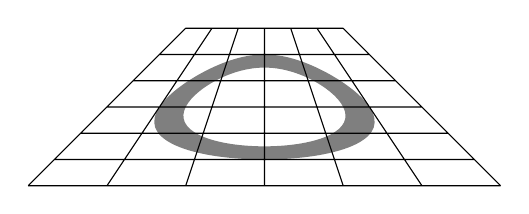
\begin{tikzpicture}
                \begin{scope}[
                grid source opposite corners={(0,0) and (6,6)},
                grid target corners={(1,1) -- (7,1) -- (5,3) -- (3,3)}]
            \pgftransformnonlinear\tikzgridtransform
            \draw (0,0) grid (6,6);
            \fill [even odd rule, opacity=0.5] 
         (3,3) circle [radius=2] circle [radius=1.5];
        \end{scope}
        \end{tikzpicture}
            }
        \caption{Perspective view.}
    \end{subfigure}%
    ~ 
    \begin{subfigure}[t]{0.5\textwidth}
        \centering
         \resizebox{.6\textwidth}{!}{%
                     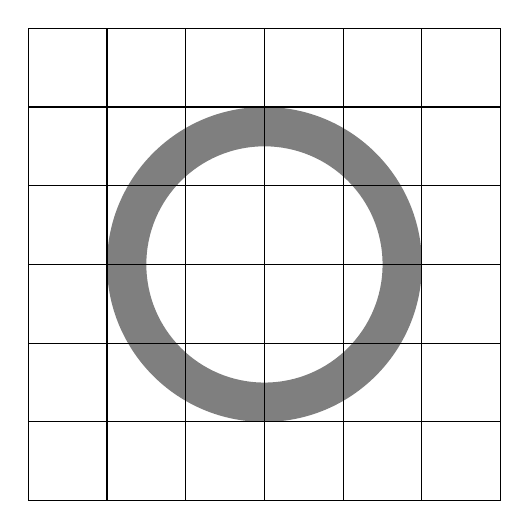
\begin{tikzpicture}                    \draw (0,0) grid (6,6);
                    %\fill [orange] (1,1) rectangle (2,2);
                        \fill [even odd rule, opacity=0.5] 
                        (3,3) circle [radius=2] circle [radius=1.5];
                    \end{tikzpicture}
            }
         \caption{Top-down view.}
    \end{subfigure}
    \caption{BEV image generated by IPM.}
    \label{fig:ipm}
\end{figure}


In general, the perspective transformation can be expressed as 
\begin{equation}
p' =  \emph{G} p
\label{eq:ipm} \; ,
\end{equation} 
where \emph{G} can be expressed in terms of the
intrinsic matrix \emph{K} and the Euclidean \emph{homography} matrix
$\emph{H} \in \mathbb{SL}(3)$ related to a planar viewed object. It should be noted that $\emph{H}$
depends on the rotation matrix $\emph{R}$ and the translation vector
$\emph{t}$ corresponds to the rigid transformation between the real camera pose image and the generated one.

IPM can be conveniently computed automatically~\cite{hom_single,adaptive_ipm} or constructed using scene measurements and satellite images from  publicly available map services (e.g. \emph{Google~Maps}).

\subsection{Object Detection}

 
 \newsavebox{\cube}
    \begin{lrbox}{\cube}
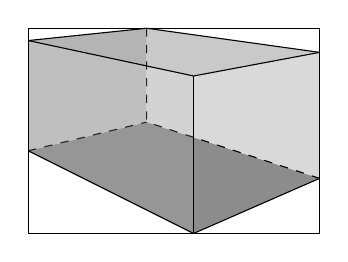
\begin{tikzpicture}
%\draw (-3,-2) grid (2,1);
%\fill [green, even odd rule, opacity=0.5] 
%(-0.5,-0.5) circle [radius=1.3] circle [radius=1];

	%%% Edit the following coordinate to change the shape of your
	%%% cuboid
      
	%% Vanishing points for perspective handling
	\coordinate (P1) at (-7cm,1.5cm); % left vanishing point (To pick)
	\coordinate (P2) at (8cm,1.5cm); % right vanishing point (To pick)

	%% (A1) and (A2) defines the 2 central points of the cuboid
	\coordinate (A1) at (0em,0cm); % central top point (To pick)
	\coordinate (A2) at (0em,-2cm); % central bottom point (To pick)

	%% (A3) to (A8) are computed given a unique parameter (or 2) .8
	% You can vary .8 from 0 to 1 to change perspective on left side
	\coordinate (A3) at ($(P1)!.7!(A2)$); % To pick for perspective 
	\coordinate (A4) at ($(P1)!.7!(A1)$);

	% You can vary .8 from 0 to 1 to change perspective on right side
	\coordinate (A7) at ($(P2)!.8!(A2)$);
	\coordinate (A8) at ($(P2)!.8!(A1)$);

	%% Automatically compute the last 2 points with intersections
	\coordinate (A5) at
	  (intersection cs: first line={(A8) -- (P1)},
			    second line={(A4) -- (P2)});
	\coordinate (A6) at
	  (intersection cs: first line={(A7) -- (P1)}, 
			    second line={(A3) -- (P2)});

    %\path let \p1=(A2) in
     %   coordinate (W1) at (0,\y1); % point on y-axis

    \path let \p1=(A5) in
        coordinate (W2) at (0,\y1); % point on y-axis


	\coordinate (C1) at
	  (intersection cs: first line={(A4) -- (A3)}, 
			    second line={(A2) -- (1em,-2cm)});
	\coordinate (C2) at
	  (intersection cs: first line={(A8) -- (A7)}, 
			    second line={(A2) -- (1em,-2cm)});
			    
	\coordinate (C3) at
	  (intersection cs: first line={(W2) -- (A5)}, 
			    second line={(A7) -- (A8)});
			    

	%%% Depending of what you want to display, you can comment/edit
	%%% the following lines

	%% Possibly draw back faces

	\fill[gray!90] (A2) -- (A3) -- (A6) -- (A7) -- cycle; % face 6
	%\node at (barycentric cs:A2=1,A3=1,A6=1,A7=1) {\tiny f6};
	
	\fill[gray!50] (A3) -- (A4) -- (A5) -- (A6) -- cycle; % face 3
	%\node at (barycentric cs:A3=1,A4=1,A5=1,A6=1) {\tiny f3};
	
	\fill[gray!30] (A5) -- (A6) -- (A7) -- (A8) -- cycle; % face 4
	%\node at (barycentric cs:A5=1,A6=1,A7=1,A8=1) {\tiny f4};
	
	\draw[thin, dashed] (A5) -- (A6);
	\draw[thin, dashed] (A3) -- (A6);
	\draw[thin, dashed] (A7) -- (A6);

	%% Possibly draw front faces

	% \fill[orange] (A1) -- (A8) -- (A7) -- (A2) -- cycle; % face 1
	% \node at (barycentric cs:A1=1,A8=1,A7=1,A2=1) {\tiny f1};
	\fill[gray!50,opacity=0.2] (A1) -- (A2) -- (A3) -- (A4) -- cycle; % f2
	%\node at (barycentric cs:A1=1,A2=1,A3=1,A4=1) {\tiny f2};
	\fill[gray!90,opacity=0.2] (A1) -- (A4) -- (A5) -- (A8) -- cycle; % f5
	%\node at (barycentric cs:A1=1,A4=1,A5=1,A8=1) {\tiny f5};

	%% Possibly draw front lines
	\draw[thin] (A1) -- (A2);
	\draw[thin] (A3) -- (A4);
	\draw[thin] (A7) -- (A8);
	\draw[thin] (A1) -- (A4);
	\draw[thin] (A1) -- (A8);
	\draw[thin] (A2) -- (A3);
	\draw[thin] (A2) -- (A7);
	\draw[thin] (A4) -- (A5);
	\draw [thin](A8) -- (A5);
	
	% Possibly draw points
	% (it can help you understand the cuboid structure)
	%\foreach \i in {1,2,...,8}
	%{
	 % \draw[fill=black] (A\i) circle (0.15em)
	%    node[above right] {\tiny A\i};
	%}
	%\draw[fill=green] (P1) circle (0.1em) node[below] {\tiny p1};
	%\draw[fill=green] (P2) circle (0.1em) node[below] {\tiny p2};

	%\draw[fill=red] (C1) circle (0.2em) node[below] {\tiny C1};
	%\draw[fill=red] (C2) circle (0.2em) node[below] {\tiny C2};
	%\draw[fill=red] (C3) circle (0.2em) node[below] {\tiny C3};
	
	%\draw[fill=green] (W1) circle (0.2em) node[below] {\tiny W1};
	
	%draw[thick, red] (A4) -- (C1);
	%\draw[thick, red] (C1) -- (C2);
	%\draw[thick] (C2) -- (A8);
    \draw[thin] (C1) rectangle (C3);
    %\draw[thick, green] (C1) rectangle ++(0.3,0.3);
\end{tikzpicture}
\end{lrbox}

\newsavebox{\icube}
    \begin{lrbox}{\icube}
\begin{tikzpicture}[scale=3.5]

	%% (A1) and (A2) defines the 2 central points of the cuboid
	% 3173
	%\coordinate (A1) at (126cm,57cm); % central top point (To pick)
	\coordinate (A1) at (127cm, 60); %68); %58cm);
	\coordinate (A2) at (140cm,4cm); % central bottom point (To pick)
	\coordinate (A3) at (117cm,21cm);
	\coordinate (A4) at (75cm,93cm); %(79cm,93cm);
	\coordinate (A5) at (97cm,127cm);
	\coordinate (A6) at (127cm,36cm);
	%\coordinate (A7) at (151cm,20cm);
	\coordinate (A7) at (151cm,19cm);
	\coordinate (A8) at (150cm, 100); %(148cm, 104); %106cm);
	
	%\coordinate (C1) at (127cm,2cm);
	\coordinate (C2) at (70cm,111cm);
	
	\coordinate (C3) at (148cm,156cm);
	\coordinate (C4) at (152cm,6cm);
	\coordinate (C1) at
	  (intersection cs: first line={(A2) -- (C4)}, 
			    second line={(A3) -- (A4)});
	\coordinate (C4) at
	  (intersection cs: first line={(A2) -- (C4)}, 
			    second line={(A8) -- (A7)});
	\coordinate (C2) at
	  (intersection cs: first line={(A5) -- (C2)}, 
			    second line={(A3) -- (A4)});
	\coordinate (C3) at
	  (intersection cs: first line={(A5) -- (C2)}, 
			    second line={(A7) -- (A8)});

	%% Possibly draw back faces

	\fill[gray!90] (A2) -- (A3) -- (A6) -- (A7) -- cycle; % face 6
	%\node at (barycentric cs:A2=1,A3=1,A6=1,A7=1) {\tiny f6};
	
	\fill[gray!50] (A3) -- (A4) -- (A5) -- (A6) -- cycle; % face 3
	%\node at (barycentric cs:A3=1,A4=1,A5=1,A6=1) {\tiny f3};
	
	\fill[gray!30] (A5) -- (A6) -- (A7) -- (A8) -- cycle; % face 4
	%\node at (barycentric cs:A5=1,A6=1,A7=1,A8=1) {\tiny f4};
	
	\draw[very thick,dashed] (A5) -- (A6);
	\draw[very thick,dashed] (A3) -- (A6);
	\draw[very thick,dashed] (A7) -- (A6);

	%% Possibly draw front faces

	% \fill[orange] (A1) -- (A8) -- (A7) -- (A2) -- cycle; % face 1
	% \node at (barycentric cs:A1=1,A8=1,A7=1,A2=1) {\tiny f1};
	\fill[gray!50,opacity=0.2] (A1) -- (A2) -- (A3) -- (A4) -- cycle; % f2
	%\node at (barycentric cs:A1=1,A2=1,A3=1,A4=1) {\tiny f2};
	\fill[gray!90,opacity=0.2] (A1) -- (A4) -- (A5) -- (A8) -- cycle; % f5
	%\node at (barycentric cs:A1=1,A4=1,A5=1,A8=1) {\tiny f5};

	%% Possibly draw front lines
	\draw[very thick] (A1) -- (A2);
	\draw[very thick] (A3) -- (A4);
	\draw[very thick] (A7) -- (A8);
	\draw[very thick] (A1) -- (A4);
	\draw[very thick] (A1) -- (A8);
	\draw[very thick] (A2) -- (A3);
	\draw[very thick] (A2) -- (A7);
	\draw[very thick] (A4) -- (A5);
	\draw[very thick] (A8) -- (A5);
	
	\draw[ultra thick] (C1) -- (C2);
	\draw[ultra thick] (C2) -- (C3);
	\draw[ultra thick] (C3) -- (C4);
	\draw[ultra thick] (C4) -- (C1);
	
	%\MarkRightAngle{A7}{A2}{A3}
\end{tikzpicture}
\end{lrbox}
 

\emph{2D object detection} is a common CV technique for identifying and locating objects of certain classes in the image.
A 2D bounding box (rectangle) is used to describe the location of an object. It is determined by the  rectangle center $c = (c_1, c_2)$, dimension $d = (d_1, d_2) $ with the width and height of the rectangle and type of the object $t \in \set{T}$.


\begin{figure}[h]
    \centering
    \begin{subfigure}[t]{0.5\textwidth}
        \centering
                 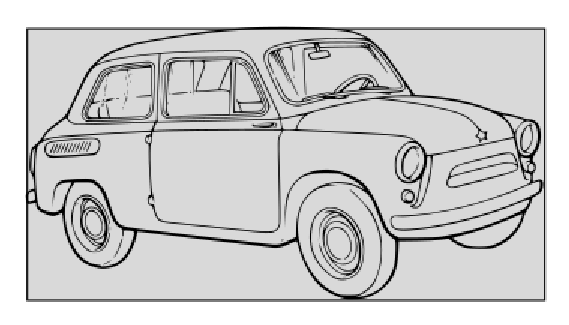
\includegraphics[width = \textwidth]{zaz_2d.eps}
        \caption{2D detection.}
    \end{subfigure}%
    ~ 
    \begin{subfigure}[t]{0.5\textwidth}
        \centering
           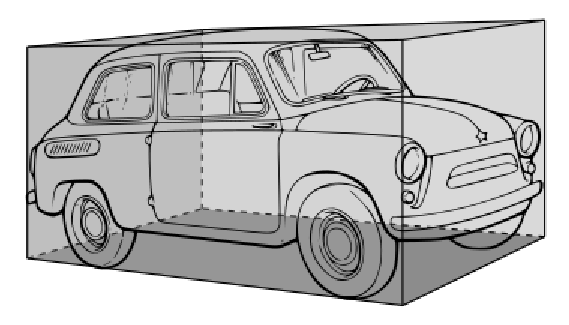
\includegraphics[width = \textwidth]{zaz_3d.eps}
         \caption{3D detection.}
    \end{subfigure}
    \caption{Vehicle detection variants.}
    \label{fig:detection}
\end{figure}

In the case of \emph{3D detection}, the bounding cuboid (or rectangular parallelepiped) is described by its 
center $c = (c_1, c_2, c_3)$, dimensions $d = (d_1, d_2, d_3)$, and
orientation $\varphi = (\varphi_1, \varphi_2, \varphi_3)$ parameterized  by elevation, azimuth and roll angles.


\section{Joint Method for 3D Detection and Instance Segmentation}  \label{sec:meth}
Instance segmentation and 3D object detection are related because they both involve identifying and localizing objects in a scene. By combining instance segmentation with 3D object detection, it is possible to obtain a more comprehensive understanding of the scene, including the shape and orientation of each individual object instance in 3D space. The basic idea of the proposed method is to find the best possible segmentation and related 3D bounding box, using the moving direction of the segment and the overage dimensions of the object.

Building a 3D box not only allows you to localize an object but, based on its dimensions, determine the most appropriate object type from the list of possibilities. We will use this observation after we construct a 2D bounding box around the segment.




\subsection{Model Assumptions}
Our main task is to detect vehicles on the road and in parking lots, but it is not limited to this application.
Several assumptions have been made in order to build a mathematical model. 
We are most interested in the planar position of the objects and  assume a
vehicle is always on flat ground. %and camera distortion is negligible.
It allows us to assume that only the azimuth (noted ${\varphi}_2$) matters and thus we do not predict the orientation $\varphi$ characterized by  elevation and roll, and we set ${\varphi}_1 = 0$ and ${\varphi}_3 = 0$.

The camera position must be stationary. In another case, object moving vectors obtained from OF have to be recalculated.
The vehicle being detected must be attached to the plane of the ground because only the points on the ground have the distance information.  



%This coincides with the definition of 3D detection and does not contradict to the \emph{Manhattan World assumption}[ref] which states that most human-made structures could be approximated by planar surfaces that are parallel to one of the three principal planes of a common orthogonal coordinate system.

%As commonly done in vehicle-oriented applications, we assume object pitch φ
%and roll α angles are zeros
In the context of our model, we consider that the shape of the objects is close to a cuboid  and also that the component parts of the object move as a whole. We use a cuboid approximation of a 3D object which coincides with the definition of 3D detection as shown in Fig.~\ref{fig:detection}.
We assume that 3D detection perfectly fits into 2D detection. Therefore, at least one vertex of the bottom box  lies on the lower side of the 2D detection rectangle. Accordingly, we can see a similar situation in BEV as shown in Fig.~\ref{fig:ipm_cube}.



Further, we will show how to find the projection of the lower face of the cuboid in  BEV.
This makes it possible to determine the center of the cuboid with known dimensions. It should be noted that the orientation of the object is determined according to the moving direction of the object and is set up to the opposite since we do not geometrically distinguish between the front and back of a vehicle, which is appropriate with cars as they can go both forwards and backwards but not sidewards.

\subsection{HSV Color Quantization} \label{sec:bbox}
 The color and shape features of an image are the most widely used features to analyze it. 
The proposed method integrates the \emph{HSV} (hue, saturation, value) color representation of the dense OF.

\begin{figure}[h]
\centering
\begin{tabular}{cc}
\subcaptionbox{Original video frame.\label{1}}{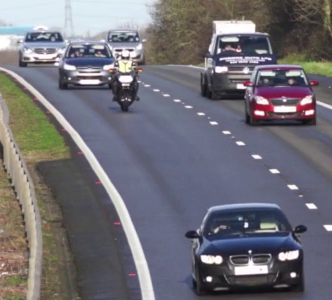
\includegraphics[width = .5\textwidth]{img/998_frame_origin.png}} &
\subcaptionbox{Dense OF visualization in HSV space.\label{2}}{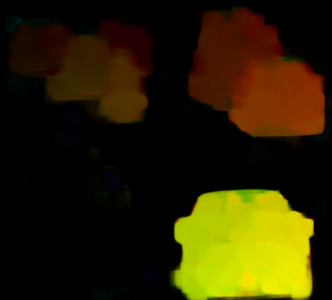
\includegraphics[width = .5\textwidth]{img/99864_flow.png}}\\

\subcaptionbox{$k = 3$ - the picture is under-segmented.\label{1}}{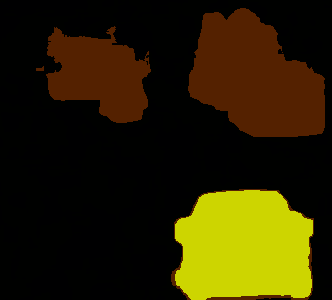
\includegraphics[width = .5\textwidth]{img/998_04_claster.png}} &
\subcaptionbox{$k = 32$ - the picture is over-segmented. \label{3}}{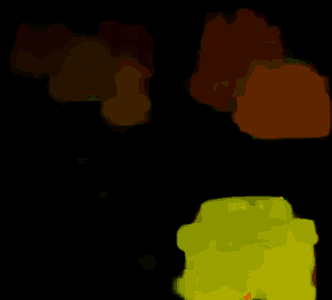
\includegraphics[width = .5\textwidth]{img/1000_32_claster.png}} 
\end{tabular}
\caption{Example of applying $k$-means clustering to dense OF.}
\label{fig:clust}
\end{figure}

%Let's consider a representation of Dense OF in HSV color space. 
For this, we visualize  the angle (direction) of flow by hue $h$ and the distance (magnitude) of flow by value $v$ with fixed saturation $s$ and then group similar colors together as shown in Fig.~\ref{fig:clust}. After applying $\mathrm{KMEANS}$ to the image $\Omega$ in HSV color space, the image will be divided into regions with fixed color values  $\overline{\Omega} = \{ \Omega_1 = (h_1, s, v_1), \dots, \Omega_k = (h_k, s, v_k) \} $.

After applying $\mathrm{KMEANS}$, each pixel in the image $\Omega$ is replaced with the color value of the nearest cluster centroid $\overline{\Omega} = \{ \Omega_1 = (h_1, s, v_1), \dots, \Omega_k = (h_k, s, v_k) \} $. 

The parameter $k$ is set so that different objects are separated (if excessive segmentation is allowed, such a value can always be chosen a-priori) as illustrated in Fig.~\ref{fig:clust}.  This is rarely sufficient for image segmentation, because there is no control over the shape of the segments. Further, we will build an iterative algorithm and a sufficiency measure that will merge the segments into one until the goal is reached.

\begin{comment}

It allows us to split off the image and compute the center, bounding rectangle, and area for each segment.

Applying $\mathrm{KMEANS}$ on pixel values corresponds to color quantization.

Of course, such a split will not define the object by default. 
   
\end{comment}

\subsection{Lifting 2D Object Detection to 3D} \label{sec:comp}
All calculations that are given in this section will refer to calculations in BEV unless it is stated otherwise. The domain of an IPM is an image with a 2D bounding box.\\

\begin{figure}[h]
    \centering
    \begin{subfigure}[t]{0.5\textwidth}
        \centering
            \resizebox{.9\textwidth}{!}{%
                 \usebox{\cube}
            }
        \caption{2D detection of a cuboid.}
    \end{subfigure}%
    ~ 
    \begin{subfigure}[t]{0.5\textwidth}
 
         \resizebox{.6\textwidth}{!}{%
            \usebox{\icube}
            }
         \caption{IPM transformation.}
    \end{subfigure}
    \caption{IPM of the 2D detection.}
    \label{fig:ipm_cube}
\end{figure}


Let the $\mathrm{IPM}$ image of a bounding rectangle  be a non-degenerate quadrangle $A, R, T, B$ with an inner rectangle where three vertices lie on adjacent sides. Moreover, one of the vertices of the rectangle lies on the bottom side of the outer quadrangle as shown in Fig.~\ref{fig:bottom}. Our goal is to find touchpoints $K, C, D$. Further, we will refer to such quadrangles as \emph{bounding} ones.

Let the rectangle be built on points $K$, $C$, and $D$ with fixed sizes $KC = a$ and $CD = b$ as shown in Fig.~\ref{fig:bottom}.
Let us draw a ray from $B$ with the angle equal to the orientation. We denote $E$ the intersection point of this ray with segment $AR$,  and $\angle ABE = \varphi$, and let $EB = l$. According to the construction  \; $\triangle K A C \backsim  \triangle E A B$ \; and 
from the similarity we have 
$\dfrac{AC}{AB} = \dfrac{KC}{EB} = \dfrac{a}{l}$ .

Hereof \; $AC = \dfrac{a}{l} (AC + CB)$ \; and \; $AC  = \dfrac{a}{l-a} CB$ \; .\\
Consequently \; $C= (C_x, C_y) = \left(\dfrac{(l - a) A_x + a  B_x}{l}, \dfrac{(l - a) A_y + a B_y}{l}\right)$ \; ,
\\which makes it possible to recover the rectangle. 

\begin{figure}[h]
    \centering

\resizebox{0.6\textwidth}{!}{%
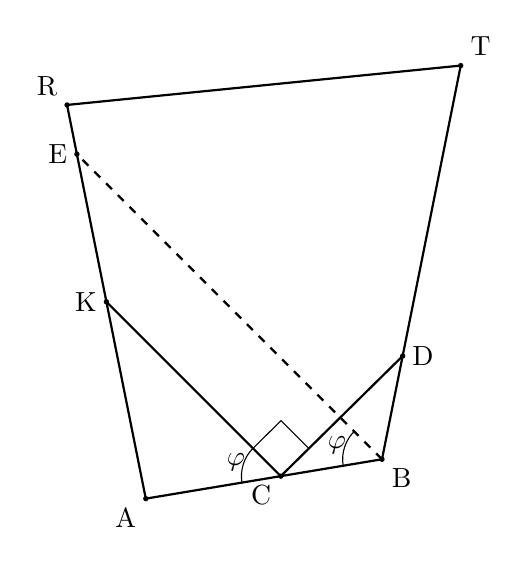
\begin{tikzpicture}[scale=0.5]

    %\draw (0,0) grid (10,15);

    \coordinate (A1) at (2cm,0cm);
    \coordinate (A4) at (8cm,1cm);
    \coordinate (A2) at (0cm,10cm); %(0cm,13cm);
    \coordinate (A3) at (10cm,11cm); %(10cm,15cm);
    
    \coordinate (K) at (0,9cm);
    \coordinate (C) at (6,0cm);
    \coordinate (C1) at (0,6cm);
    \coordinate (D) at (10,2cm);
    \coordinate (D1) at (0,13cm);
    
    \coordinate (K) at
	  (intersection cs: first line={(A4) -- (K)}, 
			    second line={(A1) -- (A2)});
			    
	\coordinate (C) at
	  (intersection cs: first line={(A1) -- (A4)}, 
			    second line={(C) -- (C1)});
	\coordinate (B) at
	  (intersection cs: first line={(C) -- (C1)}, 
			    second line={(A1) -- (A2)});
	
	\coordinate (D) at
	  (intersection cs: first line={(A4) -- (A3)}, 
			    second line={(D1) -- (D)});
			    
			    

	\draw[fill=black] (A1) circle (0.15em)
	    node[below left] { A};
	\draw[fill=black] (A4) circle (0.15em)
	    node[below right] { B};
	\draw[fill=black] (A2) circle (0.15em)
	    node[above left] { R};
	\draw[fill=black] (A3) circle (0.15em)
	    node[above right] {T};
	

    \draw[fill=black] (K) circle (0.15em) node[left] {E};
    
    \draw[fill=black] (C) circle (0.15em) node[below left] {C};
    
    \draw[fill=black] (D) circle (0.15em) node[right] {D};
    \draw[fill=black] (B) circle (0.15em) node[left] {K};


%	\draw[thick] (A1) -- (A4);
%	\draw[thick] (A4) -- (A3);
%	\draw[thick] (A3) -- (A2);
%	\draw[thick] (A1) -- (A2);


	\draw[thick] (A1) -- (A4);
	\draw[thick] (A4) -- (A3);
	\draw[thick] (A3) -- (A2);
	\draw[thick] (A1) -- (A2);
	
	\draw[thick] (C) -- (D);
	\draw[thick] (C) -- (B);
	
	\draw[thick, dashed] (A4) -- (K);

    \MarkRightAngle{D}{C}{B}
    \draw pic["$\varphi$", draw=black, -, angle eccentricity=1.2, angle radius=0.5cm]
    {angle=K--A4--C};
    

    \draw pic["$\varphi$", draw=black, -, angle eccentricity=1.2, angle radius=0.5cm]
    {angle=B--C--A1};


\end{tikzpicture}
}

    \caption{Rectangle reconstruction by angle and one side.}
    \label{fig:bottom}
\end{figure}


A rectangle with  one dimension and orientation known can be reconstructed from a bounding rectangle.\\

Since we only used one of the sides to calculate the taught-point $C$, the second side of the rectangle is calculated from Fig.~\ref{fig:bottom} as the length of segment $CD$. Therefore, the expected value $b$ may differ from the calculated one, which will be used further to determine the fitting error.\\
Returning from the bottom projection in BEV to 3D, we calculate the height of the cuboid so that the top face touches the bounding quadrilateral. The detailed analysis of the lifting procedure (we will refer to it as $\mathrm{LIFT}$) can be found in~\cite{lift}.


\subsection{Putting It All Together}
Now we are ready to describe the joint algorithm for 3D detection and instance segmentation.


\begin{figure}[h]
\centering
\begin{tabular}{cc}
\subcaptionbox{Oversized 3D box.\label{11}}{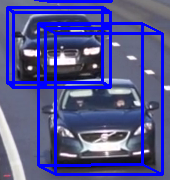
\includegraphics[width = .4\textwidth]{img/962_variant_box .png}} &
\subcaptionbox{Incorrect segmentation.\label{12}}{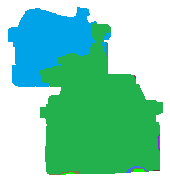
\includegraphics[width = .4\textwidth]{img/962_variant_seg.png}}\\

\subcaptionbox{Tight 3D box.\label{11}}{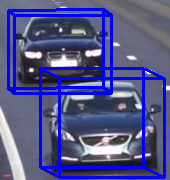
\includegraphics[width = .4\textwidth]{img/962_best_box.png}} &
\subcaptionbox{Accurate segmentation.\label{12}}{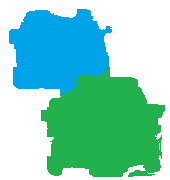
\includegraphics[width = .4\textwidth]{img/962-best_seg.png}}
\end{tabular}
\caption{Relation between 3D estimation and segmentation.}
\label{fig:relation}
\end{figure}

First of all, let's calculate an optical flow $F = \set{u = (u_1, u_2)}$ for each pixel $(x_1, x_2)$ in the video frame. We apply the $\mathrm{KMEANS}$ clustering algorithm  for the initial segmentation $\overline{\Omega} = \{ \Omega_1, \dots, \Omega_n \} $ of the image $\Omega$ , where $\Omega_i \cap \Omega_j = \varnothing $ are non-intersecting segments.
The essence of the $\Omega_i$ segment is the cluster with the closest angle and magnitude of pixels movement, as described in Fig.~\ref{fig:scheme}. Without loss of generality, we can assume that the set $\overline{\Omega}$ is sorted by area $\mathrm{S}(\Omega_{i+1}) \leq \mathrm{S}(\Omega_i)$.

Next, we will merge some segments so that they correspond to the best 3D localization -- this will be the desired instance segmentation. To do this, we choose the largest segment $\hat{\Omega}$ and build a bounding rectangle for it. Using $\mathrm{IPM}$ we find its correspondence on BEV.
Knowing the average size $d_t = (d_1, d_2, d_3)$  of the object and its orientation and type $t$, it is possible to determine the error $e$ of fitting the cuboid  with estimated center $\hat{c}$, sizes $\hat{d}$, and object type $\hat{t}$ into the bounding rectangle of the segment $\hat{\Omega}$ by error minimization:
$$ \hat{t} = \underset{t \in T}{\mathrm{argmin}} ~  \left ( \norm{d_{t} - \hat{d}} \right ), $$
where $T$ is a set of object types, and $\hat{d}$ is computed dimension.
It should be noted that in some cases it is impossible to fit the cuboid and therefore we put $e  = \infty$.\\

\begin{figure}[H]\centering 
	%the \par is necessary after each text to make the \baselineskip take effect
	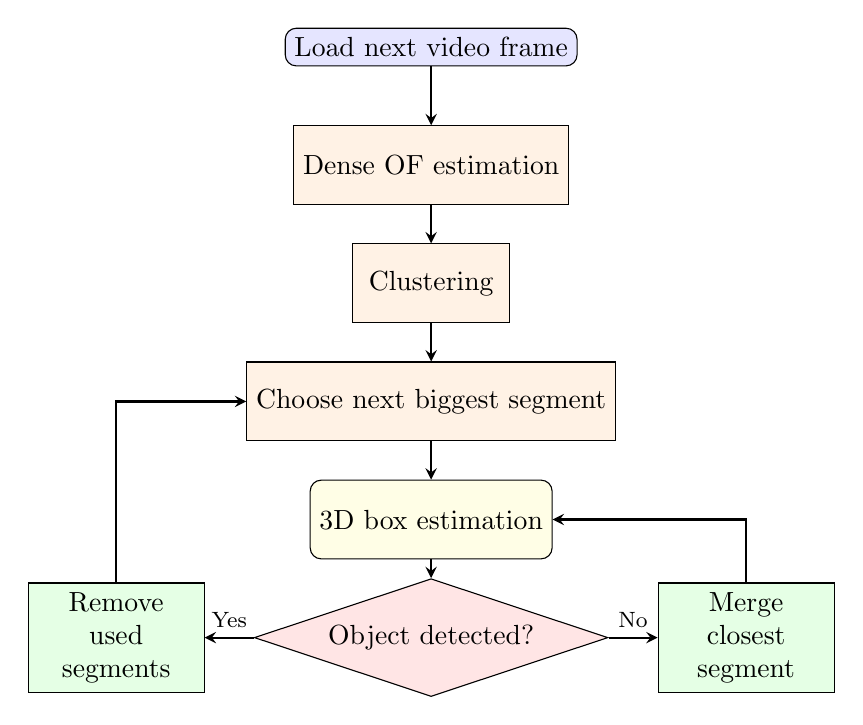
\begin{tikzpicture}[node distance=1.5 cm, auto]
	
	\node (in) [startstop] {Load next video frame \par};
	
	\node (flow) [process, below of=in] {Dense OF estimation \par };
	
	\node (seg) [process, below of=flow]{Clustering \par};

        \node (choose) [process, below of=seg]{Choose next biggest segment \par};
	\node (lift) [estimate, below of=choose]{3D box estimation \par};
	\node(detect) [decision, below of=lift]{Object detected? \par};

        \node (cycle) [compute, right of=detect, xshift=2.5cm, text width=2cm] { Merge closest segment \par };
        
        \node (remove) [compute, left of=detect, xshift=-2.5cm, text width=2cm] { Remove used segments \par };
	
	%
	

	\draw[arrow] (in) -- (flow);
	\draw[arrow] (flow) -- (seg);
	\draw[arrow] (seg) -- (choose);
        \draw[arrow] (choose) -- (lift);  
	\draw[arrow] (lift) -- (detect);
        \draw[arrow] (detect) -- (cycle) node [pos=0.5,above,font=\footnotesize]{No};
        \draw[arrow] (detect) -- (remove) node [pos=0.5,above,font=\footnotesize]{Yes};
        \draw[arrow] (cycle) |- (lift);
        \draw[arrow] (remove) |- (choose);

	
	\end{tikzpicture}
	
	\caption{Block diagram of the moving instance detection algorithm.}
	\label{fig:scheme}
\end{figure}

\begin{comment}

Next, we will merge some segments so that they correspond to the best 3D localization - this will be the desired instance segmentation. To do this, we choose the largest segment $\hat{\Omega}$ and build a bounding rectangle for it. Using $\mathrm{IPM}$ we find its correspondence on BEV.
Knowing the average size $d_t = (d_1, d_2, d_3)$  of the object and its orientation and type $t$, it is possible to determine the error $e$ of fitting the cuboid  with estimated center $\hat{c}$, sizes $\hat{d}$ and object type $\hat{t}$ into the bounding rectangle of the segment $\hat{\Omega}$ by error minimization:
$$ \hat{t} = \underset{t \in T}{\mathrm{argmin}} ~  \left ( \norm{d_{t} - \hat{d}} \right ), $$
where $T$ is a set of object types, and $\hat{d}$ is computed dimension.
It should be noted that in some cases it is impossible to fit the cuboid and therefore we put $e  = \infty$.\\
\end{comment}

Further, if the error $e$ satisfies some small threshold $\mathcal{E}$, we consider that the object of type $t$ is localized by the  3D box and segmented by $\hat{\Omega}$. Otherwise, we merge the next segment $\Omega_k$ that is  the largest in size and closest to the cluster orientation neighboring segment of cluster $\hat{\Omega}$, and repeat the $\mathrm{LIFT}$ procedure for lifting the 2D bounding box to 3D. An example of the correspondence between 3D localization and instance segmentation can be found in Fig.~\ref{fig:relation}.

In fact, we can even process objects of different types if their dimensions are different. To do this, we only choose the best segmentation and localization with the smallest embedding error as shown in Alg.~\ref{alg}.

\begin{algorithm}[h] \caption{Moving instance detection.} \label{alg}
\begin{algorithmic}[1]
\Require $\mathcal V$ \Comment{video, OF, IPM}
\State Initialize $\mathcal V\gets \set{f \mid \text{ordered set of video frames}}$
%\Repeat
\For {\text{ frame} $f \in \mathcal V $}
    \State $\Omega \gets \set{(u, v)}$ \Comment{compute flow field updates for each pixel}
    \State $\overline{\Omega} \gets \mathrm{KMEANS}(\Omega) = \{ \Omega_1, \dots, \Omega_n \} $ %\Comment{apply clustering}
    \While {$\overline{\Omega} \neq \varnothing$ }%{\text{ segment} $s \in \lfloor F \rceil $}
        \State $\hat{\Omega} \gets \varnothing$
        \Repeat
        \State $\Omega^{\star} \gets \underset{\omega \in \overline{\Omega}}{\mathrm{argmax}}~\mathrm{S}(\omega)$ 
        \State $\hat{\Omega} \gets \hat{\Omega} \cup \Omega^{\star}$
        %\State $v \gets orient(F_i)$
        \State $(\hat{c}, \hat{d}, \hat{\varphi}) \gets \mathrm{LIFT}(\hat{\Omega})$
        \State $ \hat{t} \gets \underset{t \in T}{\mathrm{argmin}} ~ \norm{d_{t} - \hat{d}}$
       \Until {$ \norm{d_{\hat{t}} - \hat{d}} > \mathcal{E}  \text{ (a small positive number)}$}
       %\Ensure $V \approx V^\pi$
        \State $\overline{\Omega} \gets \overline{\Omega}  \setminus \hat{\Omega}$
    \EndWhile
\EndFor
%\Until {$\Delta < \theta \text{ (a small positive number)}$}
\State \Return 3D boxes and related segments
\end{algorithmic}
\end{algorithm}

\begin{comment}
\begin{figure}[h!]
\centering
%\hfill
\begin{subfigure}{0.6\textwidth}
    %\raggedleft
    %\vfill
    \hfill
    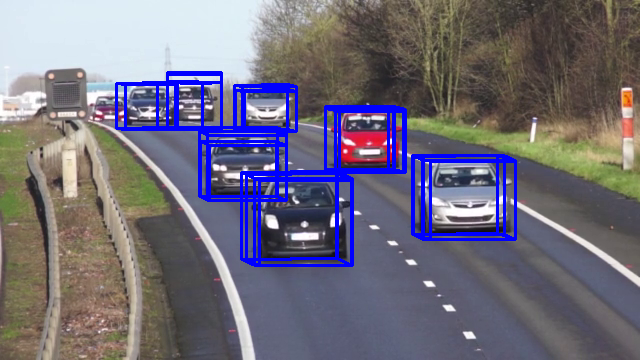
\includegraphics[height=1.8in]{img/809_box.png}
    \caption{2D YOLO detection \\with bottom projection estimation.}
    \label{fig:3d_ex}
\end{subfigure}
%\hfill
\begin{subfigure}{0.25\textwidth}
    \hfill
%\raggedright
    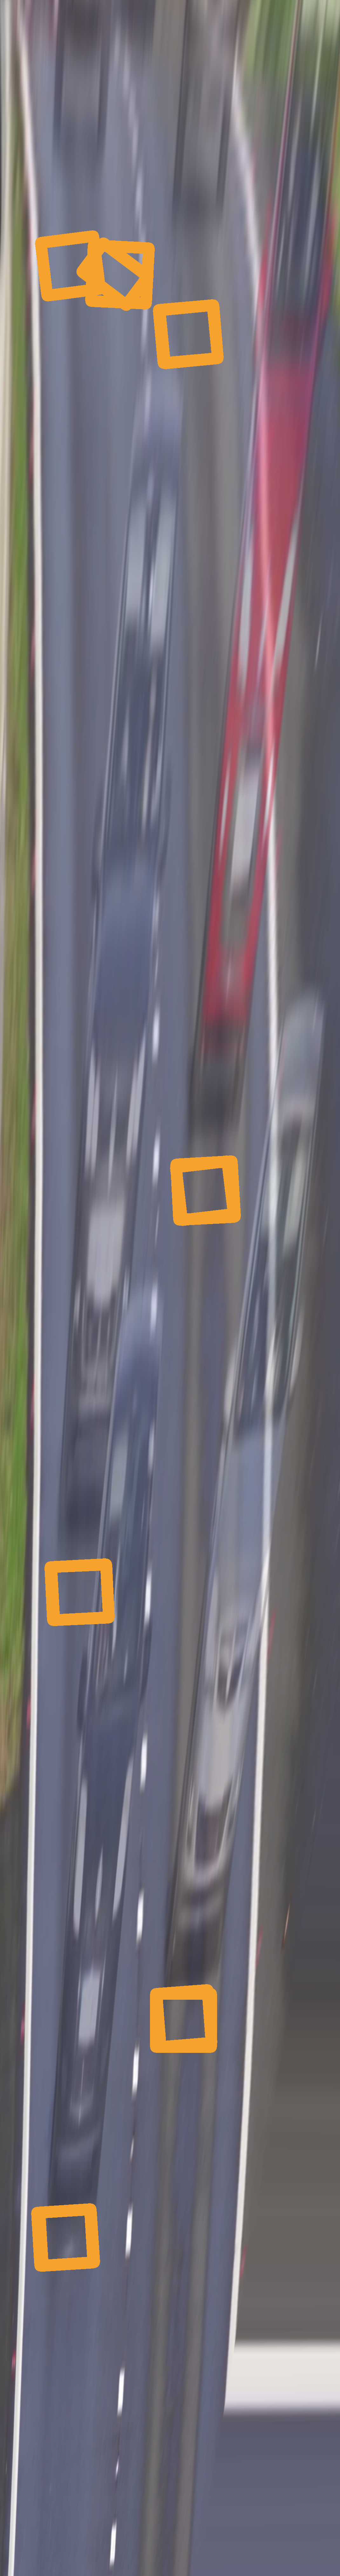
\includegraphics[height=1.8in]{img/809_bev.png}
    \caption{Related IPM\\ image.}
    \label{fig:bev_ex}
    %\hfill
\end{subfigure}
\hfill
\caption{The visualization result of the proposed 3D object detection method.}
\label{fig:met_ex}
\end{figure}
\end{comment}

An additional opportunity to avoid over-segmentation is the analysis of received bottom box projections on BEV. Firstly, the projections of the objects cannot intersect on BEV. Secondly, the segment related to the object must either be sufficiently convex, or the object must be covered by an another object that is placed closer to the camera. 
Another way to improve the results is to add tracking since the OF may not provide sufficient data for each frame to separate moving objects. The orientation and speed of moving objects cannot change randomly, because they at least should change smoothly.
Also, the most suitable type of object can be chosen from several video frames. To speed up computations, after determining the type of an object, it is possible to use it in the future without recalculation, which will limit variants during segmentation in the next video frames.

\section{Conclusion and Future Work} \label{sec:conc}


\begin{figure}[h]
\centering
\hspace{1.5em}
\begin{tabular}{cc}
\begin{subfigure}{0.81\textwidth}
%\hspace{1.5em}
\begin{tabular}{c}

\subcaptionbox{Instance segmentation based on OF.\phantom{Empty 11}\label{fig:sugseg}}{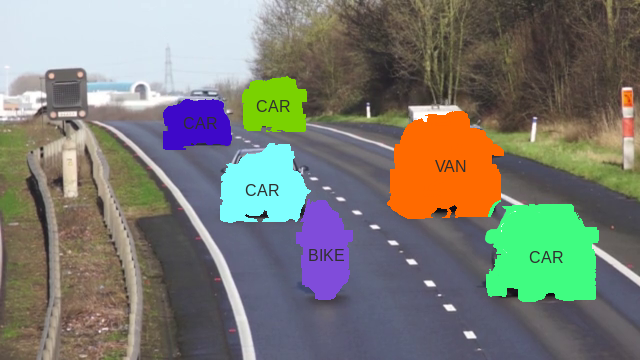
\includegraphics[width = .98\textwidth]{img/seg.png}}\\

\subcaptionbox{3D box based on segmentation.\phantom{Empty 11}\label{11}}{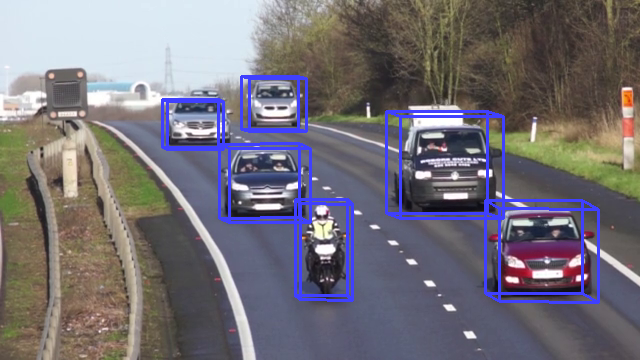
\includegraphics[width = .98\textwidth]{img/box.png}}
\end{tabular} 
\label{fig:3d_ex}
\end{subfigure} &
\hspace*{-.3em}
\begin{subfigure}{0.35 \textwidth}
   %\hfill
%\raggedright
    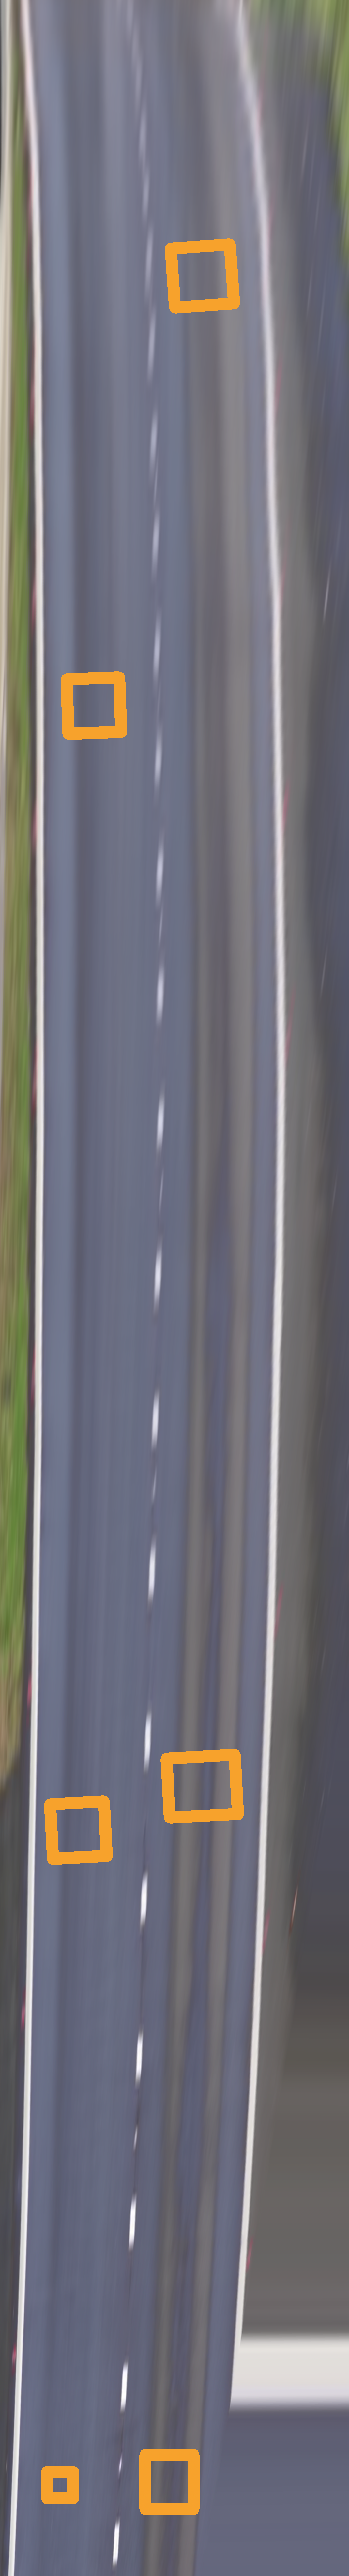
\includegraphics[width = 0.365\textwidth]{img/bev.png}
    \caption{BEV.\phantom{Projection on  Empty 111}}
    \label{fig:bev_ex}
    %\hfill
\end{subfigure}
\end{tabular}
\caption{The relation between segmentation (a), 3D box (b), and corresponding projection on BEV (c) .}
\label{fig:met_ex}
\end{figure}

In this paper, a novel approach for joint monocular 3D object detection and instance segmentation is introduced.
Despite the fact that it is based exclusively on classical methods of computer vision, it shows promising performance results.  %in speed and accuracy.
Summing up the description of the algorithm working sequence, the initial segmentation of the frame is obtained by using the clustering of the optical flow.
Then, with the help of the reconstructed 3D information from the 2D bounding box of a segment, the proposed method merges the original segments into clusters that best fit the observed objects. 
With post-processing steps, we can eliminate most of the false alarms and false positives from segmentation and 3D localization.

\begin{comment}

This article introduces an approach for a joint monocular three-dimensional detection of objects and instance segmentation.
Despite the fact that it is based exclusively on classical methods of computer vision, it is new.
This shows that methods not based on deep learning not only still remain competitive, but can also be better suited to perform tasks in conditions of limited time and resources.
In particular, the proposed method does not require training and time for learning and its behavior is completely described mathematically as the error of prediction.

In this paper, a novel approach for joint monocular 3D object detection and instance segmentation is introduced. The developed framework is promising, as it is based only on the methods of classical Computer Vision and does not require training. 
\end{comment}



Experiments have shown that the described method not only requires less time and computational resources than the deep-learning-based  algorithms,
which makes this method more applicable, but can also successfully handle overlapping objects in the image plane.
It is also possible to determine the type of objects based on their overage sizes as shown in Fig.~\ref{fig:met_ex}.

It shows that traditional methods can not only be used to solve complex modern problems but can also be better suited to perform tasks under conditions of limited time and resources.
In particular, the proposed method does not require training data and time. Its prediction error of 3D localization is fully described mathematically through the errors of the optical flow and deviations of the sizes of objects from average values.
The method is general and can be used with any optical flow and clustering algorithms.  The prospects for future studies of the non-static case with a moving camera will be considered in order to provide a 3D view for  a moving vehicle.


\begin{comment}
Testing the proposed method on video showed the wide possibilities of detection and separation of even objects whose projections intersect in a 2D image. It is also possible to determine the type of objects based on their sizes as shown in Fig.~\ref{fig:met_ex}.
\end{comment}



\begin{comment}

Using the proposed bottom box projection reconstruction method on top of dense optical flow clustering allows improvement in the accuracy and performance of the 3D object detection and segmentation. Moreover, the proposed
method also is highly adaptable, which allows it to be applied on top of any Dense OF and clustering algorithms.
Experiments  were captured on videos to test the functionality of the proposed method.
All data is processed in real-time with a high degree of accuracy~\ref{fig:met_ex}.
    
\end{comment}

\pagebreak





\section{Declarations}
\begin{itemize}
    \item The author did not receive support from any organization for the submitted work.
 \item No funding was received to assist with the preparation of this manuscript.
 \item No funding was received for conducting this study.
 \item No funds, grants, or other support was received. 
 \item  The author has no relevant financial or non-financial interests to disclose.
 \item The author has no competing interests to declare that are relevant to the content of this article.
 \item The author certifies that they have no affiliations with or involvement in any organization or entity with any financial interest or non-financial interest in the subject matter or materials discussed in this manuscript.
 \item The author has no financial or proprietary interests in any material discussed in this article.
 \item GitHub \url{https://github.com/DmitriyZhuravlev/3dim-optical-flow} 
\end{itemize}

\pagebreak

%%%%%%%%%%%%%%%%%%%%%%%% referenc.tex %%%%%%%%%%%%%%%%%%%%%
% sample references
% 
% Use this file as a template for your own input.
%
%%%%%%%%%%%%%%%%%%%%%%%% Springer%%%%%%%%%%%%%%%%%%%%%%%%%%
%
% BibTeX users please use
% \bibliographystyle{}
% \bibliography{}
%

\begin{thebibliography}{99.}%
% and use \bibitem to create references.
%
% Use the following syntax and markup for your references if 
% the subject of your book is from the field 
% "Mathematics, Physics, Statistics, Computer Science"
%
% Contribution 

\bibitem{lidar}
Shi S., Wang X., Li H.:
PointRCNN: 3D Object Proposal Generation and Detection From Point Cloud.
2019 IEEE/CVF Conference on Computer Vision and Pattern Recognition (CVPR), 2019, pp. 770-779, doi: 10.1109/CVPR.2019.00086.

\bibitem{3d_cam}
Wang Y., Zell A.:
Yolo+FPN: 2D and 3D Fused Object Detection With an RGB-D Camera.
2020 25th International Conference on Pattern Recognition (ICPR), 2021, pp. 4657-4664, doi: 10.1109/ICPR48806.2021.9413066.

\bibitem{yolo_paper}
Redmon J., Farhadi A.:
Yolov3: An incremental improvement.
arXiv preprint arXiv:1804.02767, 2018

\bibitem{traffic}
Fedorov A., Nikolskaia K., Ivanov S., Shepelev V., Minbaleev A.:
Traffic flow estimation with data from a video surveillance camera.
Journal of Big Data, vol. 6, no. 1, pp. 1–15, 2019.

\bibitem{3d_geom}
Mousavian A., Anguelov D., Flynn J., Košecká J.:
3D Bounding Box Estimation Using Deep Learning and Geometry.
2017 IEEE Conference on Computer Vision and Pattern Recognition (CVPR), 2017, pp. 5632-5640, doi: 10.1109/CVPR.2017.597.

\bibitem{lift}
Zhuravlev, D.: Lifting 2D Object Detection to 3D: Geometric Approach in Bird-Eye-View. In: Silhavy, R. (eds) Artificial Intelligence Trends in Systems. CSOC 2022. Lecture Notes in Networks and Systems, vol 502. Springer.

\bibitem{segm_trajec}
Brox T., Malik J. : Object segmentation by long-term analysis of
point trajectories. In Computer Vision–ECCV 2010, Springer, 2010, pp.
282–295.
\bibitem{segm_tracing}
Fragkiadaki K., Zhang G., Shi J. : Video segmentation by tracing
discontinuities in a trajectory embedding. In Proc. IEEE Conf. Comput. Vis. Pattern Recognit., 2012, pp. 1846–1853.

\bibitem{segm_key}
Lee Y, Kim J., Grauman K. : Key-segments for video object
segmentation. In Proc. IEEE Int. Conf. Comput. Vis., 2011, pp. 1995–
2002.
\bibitem{segm_graph}
Khoreva A., Galasso F., Hein M., Schiele B. : Classifier based graph
construction for video segmentation. In Proc. IEEE Conf. Comput. Vis.
Pattern Recognit., 2015, pp. 951–960.

\bibitem{segm_chain}
Banica D, Agape A., Ion A., Sminchisescu C. :Video object
segmentation by salient segment chain composition. In Computer
Vision Workshops (ICCVW), 2013 IEEE International Conference on,
2013, pp. 283–290.

\bibitem{segm_visual}
Papazoglou A., Ferrari V. : Fast object segmentation in
unconstrained video. Inn Computer Vision (ICCV), 2013 IEEE
International Conference on, 2013, pp. 1777–1784.

\bibitem{segm_clust}
Bandara A., Ranathunga L, Abdullah N. : Visual Feature
Clustering Using Temporal, Color and Spatial Information.
In Electronics, Communications and Networks IV (pp.677–681).

\bibitem{segm_prim}
Jang W, Lee C., Kim C. : Primary object segmentation in
videos via alternate convex optimization of foreground and background
distributions. In Proc. IEEE Conf. Comput. Vis. Pattern Recognit., 2016,
pp. 696–704.

\bibitem{segm_fusion}
Jain S., Xiong B., Grauman K. : Fusionseg: Learning to combine
motion and appearance for fully automatic segmention of generic objects
in videos. In Proc. IEEE Conf. Comput. Vis. Pattern Recognit., 2017,
pp. 3664–3673.

\bibitem{3d_geom_reduced}
Fang, J., Zhou, L., and Liu, G.:
3d bounding box estimation for autonomous vehicles by cascaded geometric constraints and depurated 2d detections using 3d results.
arXiv preprint arXiv:1909.01867, 2019.

\bibitem{bev_1}
Zhu M., Zhang S., Zhong Y., Lu P., Peng H., Lenneman J.:
Monocular 3D Vehicle Detection Using Uncalibrated Traffic Cameras through Homography.
2021 IEEE/RSJ International Conference on Intelligent Robots and Systems (IROS), 2021, pp. 3814-3821, doi: 10.1109/IROS51168.2021.9636384.

\bibitem{bev_2}
Kim Y., Kum D.:
Deep Learning based Vehicle Position and Orientation Estimation via Inverse Perspective Mapping Image.
2019 IEEE Intelligent Vehicles Symposium (IV), 2019, pp. 317-323, doi: 10.1109/IVS.2019.8814050.

\bibitem{bev_mod}
Rashed H., Essam M., Mohamed, Ei Sallab A., Yogamani S.:
BEV-MODNet: Monocular Camera based Bird's Eye View Moving Object Detection for Autonomous Driving.
2021 IEEE International Intelligent Transportation Systems Conference (ITSC), 2021, pp. 1503-1508, doi: 10.1109/ITSC48978.2021.9564667.

\bibitem{horn}
 Kanawathi J, Mokri S., Ibrahim N., Hussain A., Mustafa M.: Motion detection using Horn Schunck algorithm and implementation. 2009 International Conference on Electrical Engineering and Informatics, Bangi, Malaysia, 2009, pp. 83-87, doi: 10.1109/ICEEI.2009.5254812.

\bibitem{kmeans}
Lloyd, Stuart P.: Least squares quantization in PCM. Information Theory, IEEE Transactions on 28.2 (1982): 129-137.

\bibitem{segment}
Hafiz, A.M., Bhat, G.M.: A survey on instance segmentation: state of the art. Int J Multimed Info Retr 9, 171–
189 (2020). https://doi.org/10.1007/s13735-020-00195-x

\bibitem{fusionseg}
Jain S, Xiong B., Grauman K: Fusionseg: Learning to combine motion and appearance for fully automatic segmentation of generic objects in videos. IEEE Conference on Computer Vision and Pattern Recognition, 2017, pp. 2117–2126.



\bibitem{Hartley and Zisserman}
Hartley R., Zisserman A.:
Multiple view geometry in computer vision.
Cambridge university press, 2003

\bibitem{hom_single}
Zhou J., Li B.:
Homography-based ground detection for a mobile robot platform using a single camera.
Proceedings 2006 IEEE International Conference on Robotics and Automation, 2006. ICRA 2006., 2006, pp. 4100-4105, doi: 10.1109/ROBOT.2006.1642332.

\bibitem{adaptive_ipm} 
Jeong J., Kim A.:
Adaptive Inverse Perspective Mapping for lane map generation with SLAM.
2016 13th International Conference on Ubiquitous Robots and Ambient Intelligence (URAI), 2016, pp. 38-41, doi: 10.1109/URAI.2016.7734016.

\begin{comment}


\bibitem{kalman_mot}
Sharon M., Latha A.:
Multi-Object Tracking Based on Kalman Filter by Using Multi-Feature Appearance Model.
2018 International Conference on Inventive Research in Computing Applications (ICIRCA), 2018, pp. 544-549, doi: 10.1109/ICIRCA.2018.8597365.

\bibitem{model_det}
Ghoreyshi A., AkhavanPour A., Bossaghzadeh A.:
Simultaneous Vehicle Detection and Classification Model based on Deep YOLO Networks.
2020 International Conference on Machine Vision and Image Processing (MVIP), 2020, pp. 1-6, doi: 10.1109/MVIP49855.2020.9116922.


\bibitem{3d_mul}
Mauri A., Khemmar R., Decoux B., Haddad M., Boutteau R.:
Real-Time 3D Multi-Object Detection and Localization Based on Deep Learning for Road and Railway Smart Mobility.
J. Imaging 2021, 7, 145. https://doi.org/10.3390/jimaging7080145
\end{comment}

%
\end{thebibliography}

\end{document}
